%!TEX root = ../../main.tex
\chapter{性能評価・考察}
本研究の評価として,システムの操作性と推薦機構の評価実験を行った.

\section{システムの操作性の比較実験}
先行研究であるゴオルシェアと,私が開発しているミッションフォレストとの,操作性の比較実験を行った.

\subsection{実験内容}
サンプルとして\ref{img:experiment_question}に示すプロジェクトを提示し,ゴオルシェア及びミッションフォレスト両システムで作成してもった.
実際に作成されたツリーを,\ref{img:experiment_goalshare}と\ref{img:experiment_missionforest}に示す.
ウェブユーザビリティ評価スケール(WUS)に基づく評価項目\ref{table:experiment_question}について,どちらのシステムがよかったか,1がゴオルシェア,7がミッションフォレストとして1から7の7段階評価をしてもらった.

\begin{figure}[t]
	\begin{center}
		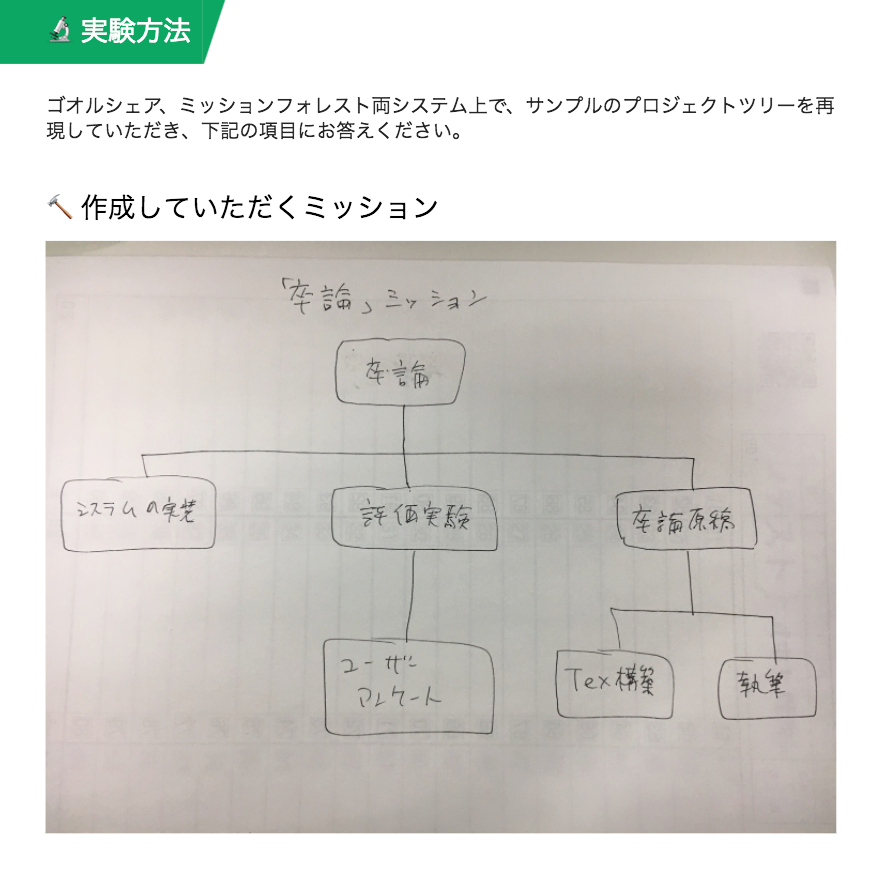
\includegraphics[width=0.9\linewidth]{assets/img/experiment_question.png}
		\caption{評価実験例題}
		\label{img:experiment_question}
	\end{center}
\end{figure}

\begin{figure}[t]
	\begin{center}
		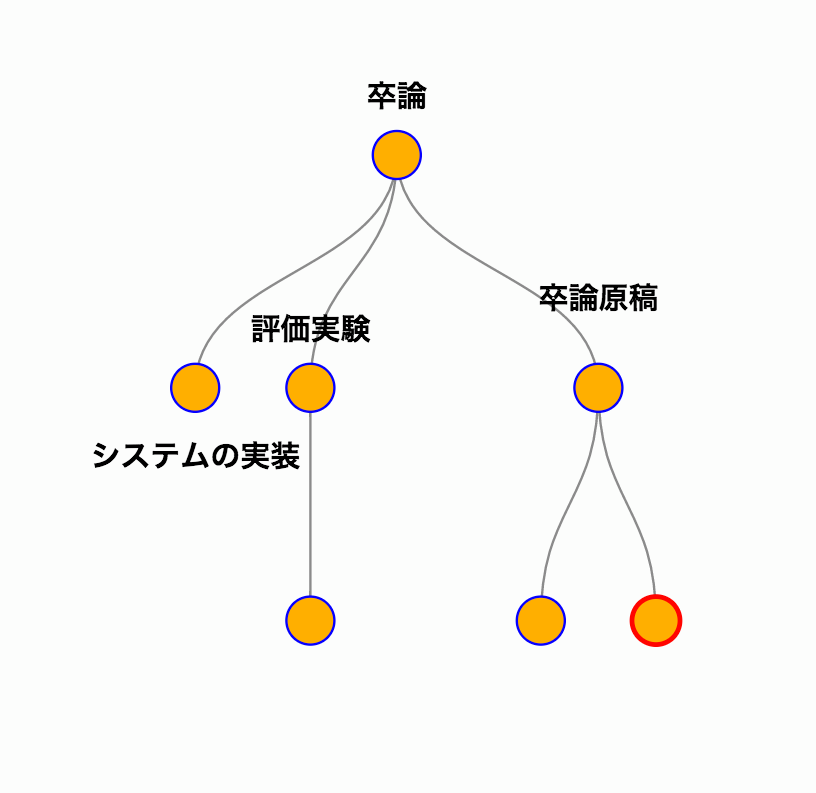
\includegraphics[width=0.9\linewidth]{assets/img/experiment_goalshare.png}
		\caption{ゴオルシェア実験結果}
		\label{img:experiment_goalshare}
	\end{center}
\end{figure}

\begin{figure}[t]
	\begin{center}
		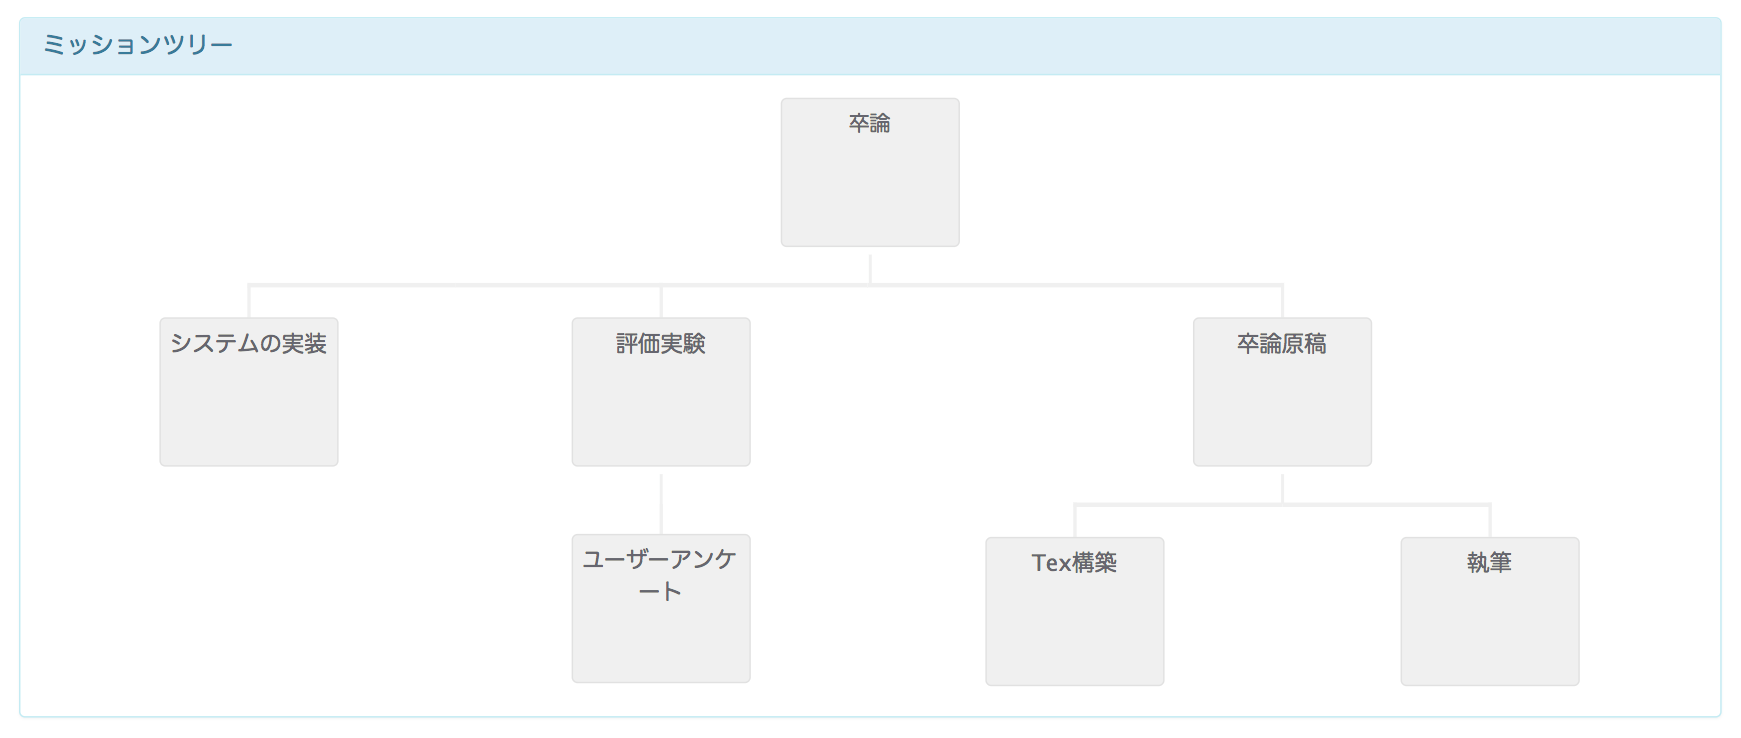
\includegraphics[width=0.9\linewidth]{assets/img/experiment_missionforest.png}
		\caption{ミッションフォレスト実験結果}
		\label{img:experiment_missionforest}
	\end{center}
\end{figure}

\begin{table}[t]
 \caption{評価実験項目}
 \begin{center}
	 \begin{tabular}{ | c | c | } \hline
		(1) & ミッションの作成はどちらが操作しやすかったですか \\ \hline
 		(2) & タスクの作成はどちらが操作しやすかったですか \\ \hline
 		(3) & 画面上のUI構成はどちらがわかりやすかったですか \\ \hline
 		(4) & どちらのツリー表示が見やすかったですか \\ \hline
 		(5) & 軽快な動きをするのはどちらでしたか \\ \hline
 		(6) & 今後どちらのシステムを使いたいですか \\ \hline
	 \end{tabular}
	 \label{table:experiment_question}
 \end{center}
\end{table}

\subsection{実験結果と考察}
今回はサンプルとして,9名の被験者に評価実験を行った.
\ref{table:experiment_result}にその解答結果を示し,それぞれの項目について信頼区間95\%で検定した結果を\ref{table:experiment_result}に示す.

\begin{table}[t]
 \caption{評価実験結果}
 \begin{center}
	 \begin{tabular}{ | c || c | c | c | c | c | c | } \hline
		  & (1) & (2) & (3) & (4) & (5) & (6) \\ \hline \hline
			被験者Aさん & 7 & 7 & 7 & 7 & 6 & 7 \\ \hline
			被験者Bさん & 7 & 6 & 6 & 5 & 6 & 6 \\ \hline
			被験者Cさん & 6 & 5 & 5 & 5 & 6 & 7 \\ \hline
			被験者Dさん & 6 & 7 & 6 & 7 & 7 & 7 \\ \hline
			被験者Eさん & 6 & 5 & 5 & 5 & 6 & 7 \\ \hline
			被験者Fさん & 7 & 7 & 6 & 6 & 6 & 6 \\ \hline
			被験者Gさん & 5 & 5 & 5 & 7 & 7 & 7 \\ \hline
			被験者Hさん & 6 & 5 & 5 & 6 & 6 & 7 \\ \hline
			被験者Iさん & 6 & 6 & 6 & 6 & 6 & 6 \\ \hline
	 \end{tabular}
	 \label{table:experiment_result}
 \end{center}
\end{table}

\begin{figure}[t]
	\begin{center}
		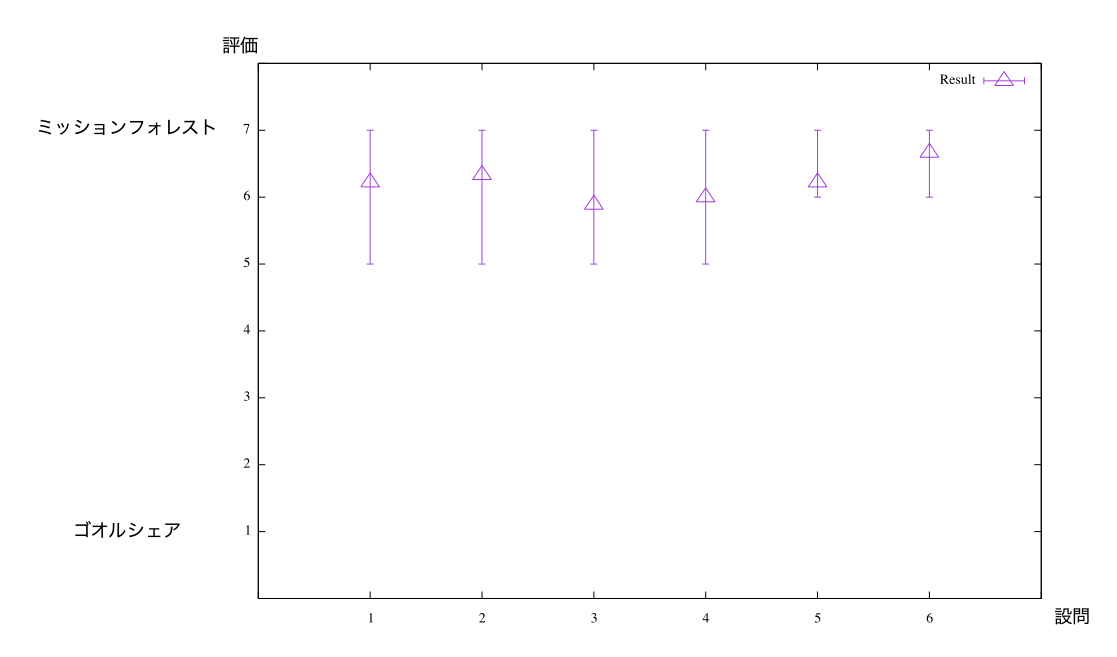
\includegraphics[width=0.9\linewidth]{assets/img/experiment_result.png}
		\caption{評価実験結果プロット}
		\label{graph:experiment_result}
	\end{center}
\end{figure}

\subsubsection{(質問1)ミッションの作成はどちらが操作しやすかったですか}
ゴオルシェアではミッション作成画面で入力項目が多すぎてわかりにくいという声が多く,
ミッションフォレストでは入力項目が少なく明確なので使いやすいという意見があった.

\subsubsection{(質問2)タスクの作成はどちらが操作しやすかったですか}
ゴオルシェアではタスクを作成するたびに画面遷移が発生していたのに対し,
ミッションフォレストでは画面遷移なしにさくさく使えるので使いやすいという意見があった.

\subsubsection{(質問3)画面上のUI構成はどちらがわかりやすかったですか}
ゴオルシェアではボタンやメニューが多く煩雑だが,
ミッションフォレストは今時のUIでシンプルだという意見があった.

\subsubsection{(質問4)どちらのツリー表示が見やすかったですか}
ゴオルシェアではタスクが丸でしか表示されないが,
ミッションフォレストではタスク名も表示されるので見やすいという意見があった.

\subsubsection{(質問5)軽快な動きをするのはどちらでしたか}
ゴオルシェアでは画面遷移のたびに待ち時間があったが,
ミッションフォレストでは画面遷移がないので待ち時間が短いという意見があった.

\subsubsection{(質問6)今後どちらのシステムを使いたいですか}
タスクの作りやすさとツリーの見やすさから,ミッションフォレストを使いたいという意見が多かった.
